% This is the aspauthor.tex LaTeX file
% Copyright 2010, Astronomical Society of the Pacific Conference Series

\documentclass[11pt,twoside]{article}
\usepackage{./asp2010}

\resetcounters

\bibliographystyle{asp2010}

\markboth{Sick, Courteau and Cuillandre}{Andromeda Optical \& Infrared Disk Survey}

\begin{document}

\title{The Andromeda Optical and Infrared Disk Survey}
\author{Jonathan Sick,$^1$ St\'{e}phane Courteau,$^1$ and Jean-Charles Cuillandre$^2$}
\affil{$^1$Queen's University, Kingston Ontario Canada K7L 3N6}
\affil{$^2$Canada-France-Hawaii Telescope Corporation}

\begin{abstract}
The Andromeda Optical and Infrared Disk Survey has mapped M31 in $u^* g^\prime r^\prime i^\prime J K_s$ wavelengths out to $R=40$~kpc using the MegaCam and WIRCam wide-field cameras on the Canada-France-Hawaii Telescope.
Our survey is uniquely designed to simultaneously resolve stars while also carefully reproducing the surface brightness of M31, allowing us to study M31's global structure in the context of both resolved stellar populations and spectral energy distributions.
We use the Elixir-LSB process to subtract backgrounds from the optical $u^* g^\prime r^\prime i^\prime$ images by building real-time maps of the sky background with sky-target nodding.
These maps are stable to $\mu_g \lesssim 28.5$~mag~arcsec$^{-2}$ and reveal warps in the outer M31 disk in surface brightness.
The equivalent mapping in the Near-Infrared with WIRCam uses a combination of sky-target nodding and image-to-image sky offset optimization to produce stable surface brightnesses, although a surface brightness zeropoint calibration using resolved stellar population is also required.
A key application of this data set is to understand the systematics of spectral energy distribution fitting with near-infrared bands where asymptotic giant branch stars impose a significant, but ill-constrained, contribution to the near-infrared light of a galaxy.
Here we present our panchromatic surface brightness maps of M31 and initial results from our near-infrared resolved stellar catalog.
\end{abstract}

\section{Introduction to the ANDROIDS Project}

The Andromeda Galaxy (M31) is a special laboratory for testing our understanding of galaxy formation and evolution.
Its close proximity enables detailed mapping of the star formation histories imprinted in resolved stellar populations, while our external vantage permits detailed decompositions of galaxy structures.
Here we present the Andromeda Optical and Infrared Disk Survey (ANDROIDS): a homogeneous mapping of the entire Andromeda Galaxy from near-UV to near-infrared wavelengths with imaging that simultaneously resolves stars and accurately recovers surface brightness.
This survey is being carried out with the MegaCam ($u^*g^\prime r^\prime i^\prime$) and WIRCam ($JK_s$) instruments on the Canada-France-Hawaii Telescope.
ANDROIDS improves upon previous all-disk star catalogs \citep[e.g., the Local Group Galaxy Survey][]{Massey:2006} with improved seeing, superior $u^*$ sensitivity and incorporation of NIR bands.
Previous surface brightness investigations of the M31 disk have either been confined to just encompass the 10~kpc star forming ring in SDSS optical imaging \citep{Tamm:2012} or to just the bulge in 2MASS NIR imaging \cite{Beaton:2007}.
The ANDROIDS survey uses rigorous background subtraction strategies to obtain robust surface brightness measurements out to $R=40$~kpc along the disk.

A prime motivation for the ANDROIDS survey, besides mapping M31's structure and stellar content, is to understand the systematics of stellar population synthesis, particularly in the near-infrared.
Combining near-infrared (NIR) and optical data is invaluable for alleviating the well-known degeneracy between the stellar metallicity, age and dust content on a galaxy's colors.
Near-infrared observations are also attractive for estimating the stellar mass of because they are nearly unattenuated by dust, while also being sensitive to lower mass mass that dominate a galaxy's mass.
However, the wide-spread use of near-infrared bands has been stunted by our inability to consistently include them in spectral energy distribution (SED) fits.
For example, \cite{Taylor:2011} have found that SED fits to optical-NIR data sets have much larger residuals than optical-only fits.
Consequently, \cite{Zibetti:2009}, \cite{Taylor:2011} and others advocate ignoring NIR data in stellar mass estimation and instead rely upon $g-i$ colors.
There are two options for resolving issues with NIR SEDs.
First, the because the inclusion of NIR bands breaks degeneracies, our parameterizations of star-formation histories may be too simplistic.
Note that is it common to fit galaxy SEDs with a single-metallicity stellar population and a parametric star formation rate; perhaps the NIR data begs for multiple metallicity components, complex star formation rate histories and more realistic dust models.
A second possibility is that stellar population synthesis itself is unreliable at NIR wavelengths.
This is entirely plausible if we realize that the dominant contributors of NIR light are actually asymptotic giant branch (AGB) stars whose fleeting evolution is extremely difficult to model.
The ANDROIDS survey is well suited to pointing out tensions in NIR stellar population synthesis since a region's SED can be measured, while the resolved stars that contribute to that SED are also measured.

\section{Low Surface Brightness Imaging of M31}

\begin{figure}[t]
\centering
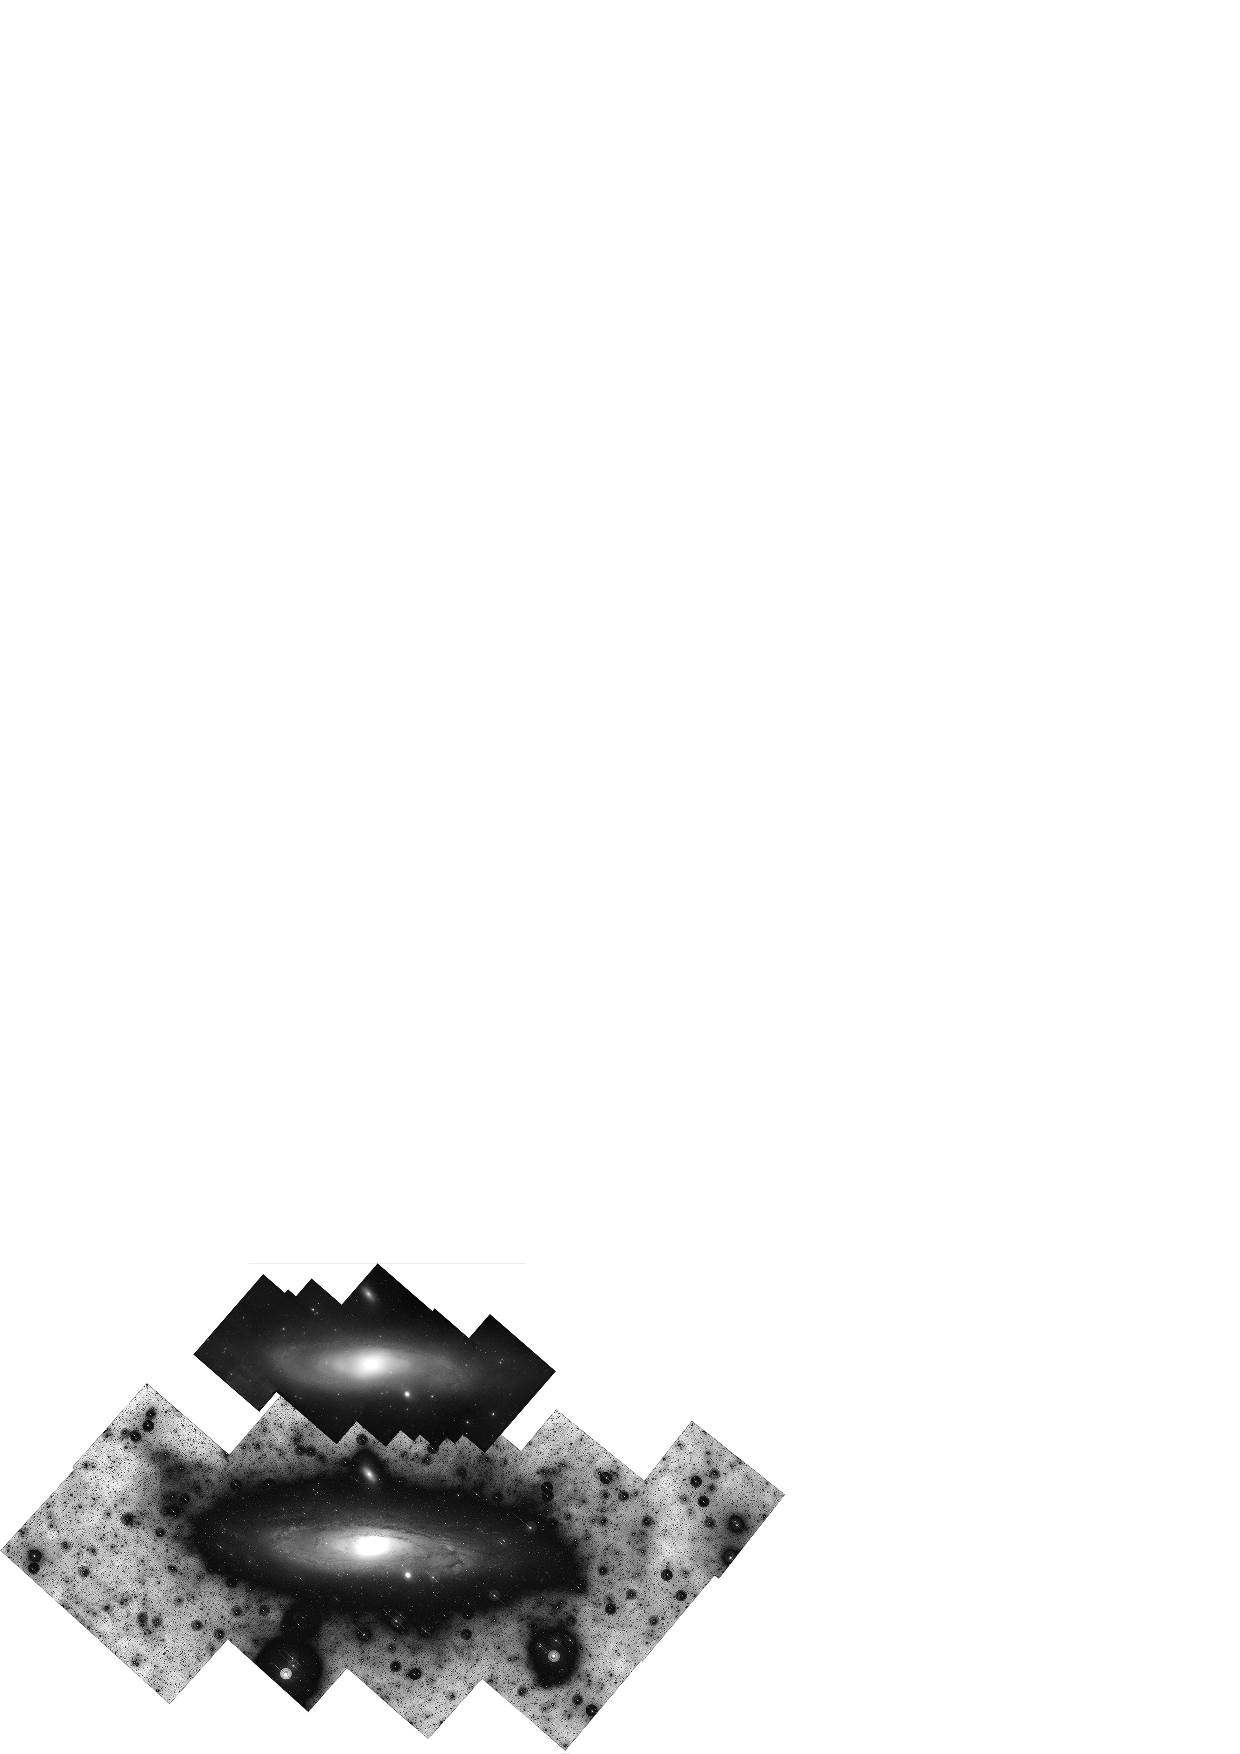
\includegraphics[width=\columnwidth]{mosaics}
\caption{ANDROIDS $J$-band mosaic (top) and MegaCam mosaics (bottom).}
\label{fig:mosaics}
\end{figure}

Accurate surface brightness mapping is a unique quality of our ANDROIDS survey that is neglected by previous surveys.
Covering the Andromeda Galaxy's disk requires fourteen 1-square degree pointings with MegaCam.
Thus the background signal cannot be directly known from a field on the disk, yet calibration systematics must be precisely controlled to avoid error propagation across the maps.
For our CFHT/MegaCam optical mapping we have used a new process called Elixir-LSB that allows us to calibrate the surface brightness in an instrument that has previously been optimized for point-source surveys.
The basic feature of the Elixir-LSB process is real-time background monitoring, which we do by covering with ANDROIDS footprint in a sky-target-target-sky nodding pattern with seven unique sky fields.
We image the entire footprint in a period of 1~hour with a sky-target-target-sky nodding pattern that allows us to maintain a model of the background from a moving window of sky observations.
This process is similar to the background subtraction done for NIR observations.
The result is optical mosaics with modest integrations per field (15~minutes in $g^\prime r^\prime i^\prime$, 45~minutes in $u^*$) that reach surface brightness levels of $\mu_g \lesssim 28.5$~mag~arcsec$^{-2}$, while also having a pixel scale of 0.7~pc on the disk of M31.
In Fig.~\ref{fig:mosaics} we present the ANDROIDS optical mosaics.
We have stretched the colour mapping in the outer disk to show that we have a stable surface brightness calibration out to the mosaic edge at $R=40$~kpc along the major axis.
For the first time, the Northern spur in the M31 disk is seen in \emph{integrated} light, after first being detected by \cite{Ferguson:2002} in stellar density maps.
Halos around foreground stars are the main sources of surface brightness contamination in our maps, but can be easily masked.
The MegaCam $u^*g^\prime r^\prime i^\prime$ mosaics of M31 will enable studies of M31's structure, stellar mass and populations and dust content using the same tools that have been developed for more distant galaxies.

Producing equivalent surface brightness maps at $J$ and $K_s$ is far more difficult, as outlined by \cite{Sick:2013}.
The near-infrared sky glow is both bright, $10^3\times$ M31's NIR surface brightness at $R=20$~kpc, and variable in space and time.
Although we attempted several sky-target nodding strategies, \cite{Sick:2013} find that nodding across a target as large as M31 introduces background level uncertainties at a level of 2\% of the NIR background.
By solving for a set of background level offsets for each image that minimize image-to-image surface brightness discontinuities, we are able to get produce NIR mosaics that are stable to $< 0.1$\% of the background level.
% The mosaics are limited by variations in the background shape with amplitudes of 0.2\% of the background level across a WIRCam frame.
Since our background corrections are so large, $>1$\% of the NIR background level, our mosaics are subject to a zeropoint uncertainty that grows to 0.2~mag~arcsec$^{-2}$ at $R=15$~kpc.
The absolute surface brightness, however, can be calibrated by appealing to the surface brightness of resolved stars.

\section{Near-Infrared Stellar Populations}

\begin{figure}[t]
\centering
\includegraphics[width=\columnwidth]{cmd}
\caption{Near-infrared color magnitude diagrams of a field on the M31 disk major axis at $R=20$~kpc (right) and in the outer disk (left). Padova isochrones are over plotted with $\log Z/Z_\odot=0.2$ metallicity for various ages.}
\label{fig:cmd}
\end{figure}

We also present initial results from the ANDROIDS NIR resolved stellar catalog, an overview of which we present in Fig.~\ref{fig:cmd}.
A great advantage of NIR photometry of M31 is that NIR sequences have distinct colours compared to the Milky Way foreground that has $J-K_s < 0.8$.
Optical colours of post-main sequence M31 stars, on the other hand, tend to lie in the Milky Way color distribution, making foreground removal nearly impossible.
Indeed, this is why previous resolved stellar population analyses of M31 \citep[e.g.,][]{Williams:2003,Davidge:2012} have been restricted to young ($<500$~Myr) populations.

In the outer disk, our CMDs are complete $>1$~mag below the tip of the red giant branch (RGB).
Our ANDROIDS NIR colour magnitude diagrams are sensitive to asymptotic giant branch (AGB) and upper RGB in M31.
In Fig.~\ref{fig:cmd} we plot Padova high metallicity ($\log Z/Z_\odot = 0.2$) isochrones \citep{Marigo:2008} against a $J-K_s$ CMD of a field at 20~kpc along the northern major axis.
Near-infrared RGB and AGB sequences become dimmer and only slightly redder with increasing age and become redder with increasing metallicity and dust content.
We find that our outer-disk NIR stellar populations are consistent with predominantly intermediate-age ($>1$~Gyr) high-metallicity population.
This agrees with HST observations by \cite{Brown:2006}.
Stars in the disk-halo transition are nearly mono-abundance, while those in the outer optical disk are redder than expected, likely due to additional extinction.

\section{Future Work}

The intention of the ANDROIDS survey is to become a reference a panchromatic, optical to NIR, reference for the SED, structure and resolved stellar populations of M31's entire disk within $R=40$~kpc.
This work is synergistic with the Panchromatic Hubble Andromeda Treasury Survey \citep[PHAT;][]{Dalcanton:2012} which has higher-resolution imaging of one quadrant of the M31 disk in a similar wavelength range, and the Pan-Andromeda Archaeological Survey \citep[PAndAS;][]{McConnachie:2009} which has mapped M31's stellar halo with $g^\prime i^\prime$ imaging.
In future work we will exploit our mapping to understand the stellar mass decomposition in the M31 disk, halo and bulge.
With resolved stellar populations, and where confusion in the disk becomes too high, SEDs, we will map star formation histories and dusk content in M31.
And by confronting panchromatic SED fitting with resolved stellar populations, we will identify the tensions in near-infrared stellar population synthesis.

\acknowledgements We thank Marc Seigar for organizing a wonderful conference, and the other attendees for enlightening discussions. We also thank ANDROIDS team members M.~McDonald, R.~S. de~Jong and R.~B.~Tully for their work in kick starting the survey.

\bibliography{sickj}

\end{document}
